
\documentclass[12pt]{article}
\usepackage{graphicx}
\usepackage{amsmath}
\usepackage{hyperref}
\usepackage{geometry}
\geometry{margin=1in}
\title{Frequency-Domain Logic Encoding for Protocol-Enforced Systems}
\author{Christopher Hirschauer \\ \texttt{c.hirschauer@outlook.com}}
\date{August 30, 2025}

\begin{document}
\maketitle
\begin{abstract}
This paper proposes a novel control architecture that replaces traditional binary logic with frequency-domain encoding to achieve enhanced semantic density, forensic traceability, and protocol-level enforcement. By mapping logical states to discrete frequency bands, the system enables multi-valued logic, intent encoding, and resilient plugin validation. The tradeoff between raw execution speed and semantic throughput is quantified, and implementation pathways are outlined for both software simulation and hardware integration.
\end{abstract}

\textbf{Keywords:} protocol-based computing, frequency-domain logic, semantic encoding, control architecture, auditability

\section{Introduction}
Traditional computing systems rely on binary logic—voltage levels representing 0 and 1—to encode and execute instructions. While efficient, this model lacks semantic expressiveness and is vulnerable to default behaviors, abstraction leakage, and audit failure. This paper introduces a frequency-based logic model where each logical state is represented by a distinct frequency, enabling multi-bit encoding per signal pulse and enforcing control protocols at the signal layer.

\section{Frequency-Based Logic Model}
\subsection{Encoding Scheme}
\begin{itemize}
  \item Binary Model: 2 frequencies → 1 bit per pulse
  \item Hex Model: 16 frequencies → 4 bits per pulse
  \item Extended Model: $2^n$ frequencies → $n$ bits per pulse
\end{itemize}
Each frequency $f_i$ maps to a semantic intent:
\begin{itemize}
  \item $f_1 = 1$ kHz → Audit-only
  \item $f_{10} = 10$ kHz → Override Approved
  \item $f_{16} = 16$ kHz → Force Rollback
\end{itemize}

\subsection{Control Enforcement}
Execution is gated by frequency validation. Instructions are only executed if the correct frequency signature is present, ensuring explicit approval and forensic traceability.

\section{Semantic Throughput vs Raw Speed}
\subsection{Semantic Gain}
Hex-frequency encoding delivers 4x semantic payload per signal compared to binary. Reduces signal count per instruction by 50%.

\subsection{Speed Tradeoff}
Signal discrimination latency: ~30–50\% overhead. Synchronization and filtering introduce MHz-scale bottlenecks. Net result: slower execution, but higher control fidelity.

\section{Implementation Pathways}
\subsection{Software Simulation}
Python-based signal generator using \texttt{numpy} and \texttt{scipy.signal}:
\begin{verbatim}
import numpy as np
from scipy.signal import chirp
import matplotlib.pyplot as plt

fs = 100000  # Sampling frequency
T = 1        # Duration in seconds
f_start = 1000
f_end = 16000

t = np.linspace(0, T, int(fs*T))
signal = chirp(t, f0=f_start, f1=f_end, t1=T, method='linear')

plt.figure(figsize=(10, 4))
plt.plot(t, signal)
plt.title('Frequency-Encoded Signal')
plt.xlabel('Time [s]')
plt.ylabel('Amplitude')
plt.grid(True)
plt.tight_layout()
plt.savefig('frequency_encoded_signal.png')
\end{verbatim}
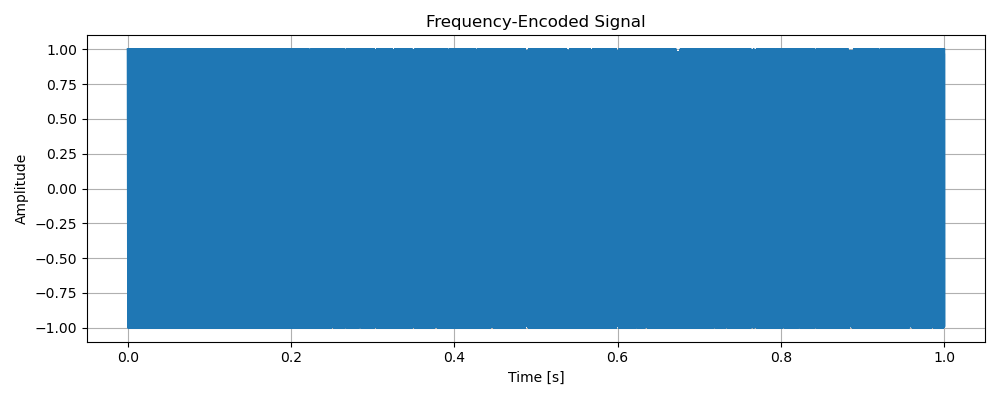
\includegraphics[width=\textwidth]{frequency_encoded_signal.png}

\subsection{Hardware Integration}
\begin{itemize}
  \item FPGA or DSP-based frequency discriminators
  \item Oscillator banks for signal generation
  \item Analog-to-digital converters for real-time validation
\end{itemize}

\section{Error Modeling and Resilience}
Frequency misclassification modeled via Gaussian noise and band overlap. Error correction via Hamming codes or CRC tagging. Redundant fallback frequencies for recovery modes.

\section{Applications}
\begin{itemize}
  \item Plugin Recovery Protocols: Frequency-tagged rollback and override signals
  \item AI Instruction Enforcement: GPT directives encoded in waveform pulses
  \item Forensic Logging Systems: Signal-level audit trails with semantic tagging
\end{itemize}

\section{Conclusion}
Frequency-domain logic encoding offers a transformative approach to control architecture, enabling multi-valued logic, semantic compression, and protocol-level enforcement. While it introduces latency, the tradeoff is justified in systems demanding resilience, auditability, and override protection. This model redefines the relationship between signal and intent, paving the way for next-generation protocol-driven computing.

\bibliographystyle{plain}
\bibliography{protocol_computing_references}
\end{document}
